\documentclass[tikz,border=2pt]{standalone}
\usepackage{amsmath,amssymb}
\usepackage{tikz}
\usetikzlibrary{arrows.meta}

\begin{document}
% m is a lower bound of S when every element of S lies at or to the right of m; the greatest
% lower bound is the infimum.
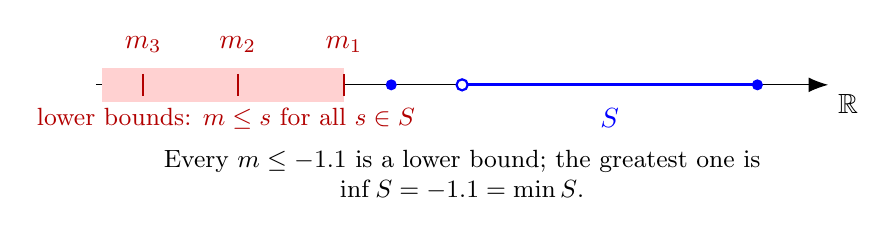
\begin{tikzpicture}[x=1.5cm]
	\draw[-{Latex[length=2.5mm]}] (-3.6,0) -- (2.6,0) node[below right] {$\mathbb{R}$};
	\fill[red!18] (-3.55,-0.22) rectangle (-1.5,0.22);
	\draw[very thick, blue] (-0.5,0) -- (2,0);
	\draw[blue, thick, fill=white] (-0.5,0) circle (2pt);
	\fill[blue] (2,0) circle (2pt);
	\fill[blue] (-1.1,0) circle (2pt);
	\node[blue, below=5pt] at (0.75,0) {$S$};
	\foreach \x/\l in {-1.5/$m_1$, -2.4/$m_2$, -3.2/$m_3$} {\draw[red!70!black, thick] (\x,0.14) -- (\x,-0.14); \node[red!70!black, above=4pt] at (\x,0.14) {\l};}
	\node[red!70!black, below=5pt, font=\small] at (-2.5,0) {lower bounds: $m\le s$ for all $s\in S$};
	\node[anchor=north, align=flush center, text width=10cm, font=\small] at (-0.5,-0.7) {Every $m\le -1.1$ is a lower bound; the greatest one is $\inf S=-1.1=\min S$.};
\end{tikzpicture}
\end{document}
